% Drawing 154/02-20 -- folder 154, batch 02, archive page 31 (PDF page 32).
% Transcription: figure à gauche des formules : deux arêtes fléchées vert foncé et deux vert clair, se croisant ; $s$ en bas à droite, $t$ en haut ; un losange au crayon, hachuré dans sa moitié inférieure, dont les quatre repères sont marqués $r$, $\sigma_0 r$, $\sigma_1 r$, $\sigma_2 r$ ; une petite flèche courbe tourne autour de $s$
% Kind: flags around two crossing arrowed edges. Method 2 (schematic redraw from the facsimile). Status: ok.
% Notes: Four arrows: light green from s up to t, light green from s down to the left, dark green leftwards across the first, dark green upwards across the second; the pencil lozenge joins their ends, its lower part hatched; labels r in the middle, sigma_2 r on its right, sigma_1 r below (overwritten on the page), and above the one read sigma_0 r by elimination (its index is not legible). Redrawn 2026-11-12 (issue 128): to check again.
% Coordinates: 1 unit = 1 mm = 1/100 of the crop width (bbox in page fractions: [0.525, 0.19, 0.66, 0.315]).
% Redrawn by Claude (claude-fable-5-2), issue #128, 2026-11-12; not checked by a human; not compiled (no TeX in the session).
% Rights: reproduces part of the work -- behind RENDER_TRANSCRIPTS, never published by itself.
\documentclass[tikz,border=3pt]{standalone}
\usepackage{amsmath,amssymb}
\usetikzlibrary{patterns,arrows.meta}
\tikzset{Lg/.style={green!60!black!70}, Dg/.style={green!45!black}, pencil/.style={black!45}, struck/.style={black!35}, mpt/.style={circle,draw,inner sep=1.3pt}, pt/.style={circle,fill,inner sep=0.9pt}, opt/.style={circle,draw,fill=white,inner sep=1.1pt}}
\begin{document}
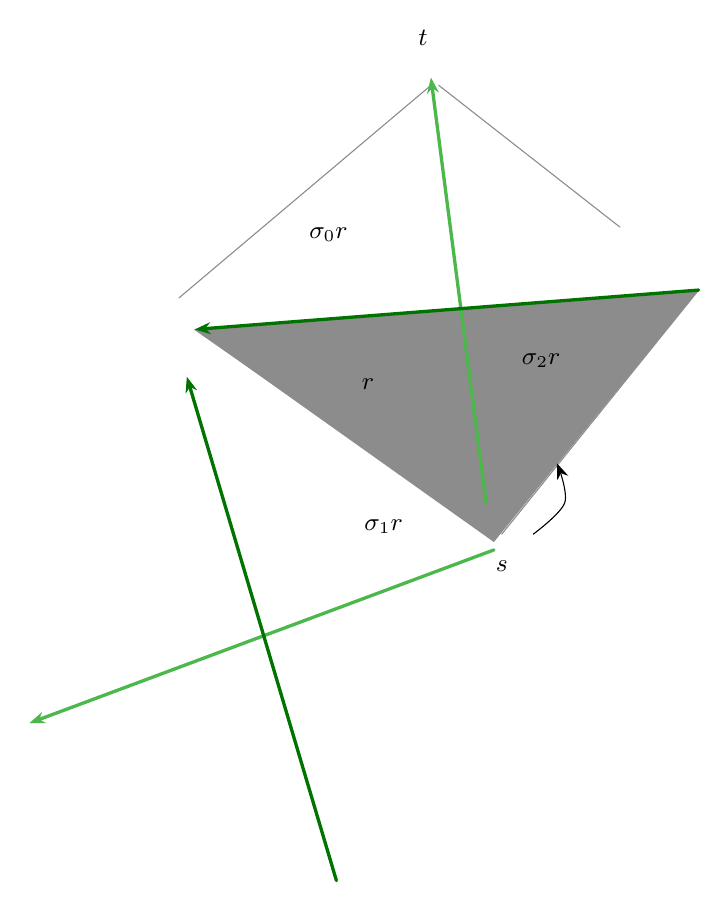
\begin{tikzpicture}[x=1mm,y=1mm,line cap=round,line join=round,font=\scriptsize]
\fill[pattern=north east lines,pencil] (33,-58) -- (66,-55.5) -- (97,-53) -- (71,-85) -- cycle;
\draw[pencil] (63,-27) -- (31,-54);
\draw[pencil] (64,-27) -- (87,-45);
\draw[pencil] (33,-58) -- (69,-83);
\draw[pencil] (97,-53) -- (72,-84);
\draw[Lg,very thick,-{Stealth[length=2mm]}] (70,-80) -- (63,-26);
\draw[Lg,very thick,-{Stealth[length=2mm]}] (71,-86) -- (12,-108);
\draw[Dg,very thick,-{Stealth[length=2mm]}] (97,-53) -- (33,-58);
\draw[Dg,very thick,-{Stealth[length=2mm]}] (51,-128) -- (32,-64);
\draw[-{Stealth[length=2mm]}] plot[smooth, tension=0.55] coordinates {(76,-84) (80,-80) (79,-75)};
\node[inner sep=1pt] at (62,-21) {\small $t$};
\node[inner sep=1pt] at (72,-88) {\small $s$};
\node[inner sep=1pt] at (50,-46) {\small $\sigma_0 r$};
\node[inner sep=1pt] at (55,-65) {\small $r$};
\node[inner sep=1pt] at (77,-62) {\small $\sigma_2 r$};
\node[inner sep=1pt] at (57,-83) {\small $\sigma_1 r$};
\end{tikzpicture}
\end{document}
